\section{Introduction}


\begin{frame}{Introducing Myself}
    \begin{columns}
        % Column 1
        \begin{column}{0.5\textwidth}
            \begin{itemize}
                \item Isak Hammer, 27 year old, Lofoten
                \item Graduate student in Industrial Mathematics
                \item Research Focus: Numerical methods for Partial Differential Equations (PDEs).
            \end{itemize}
        \end{column}

        % Column 2
        \begin{column}{0.5\textwidth}
            \begin{figure}
                \centering
                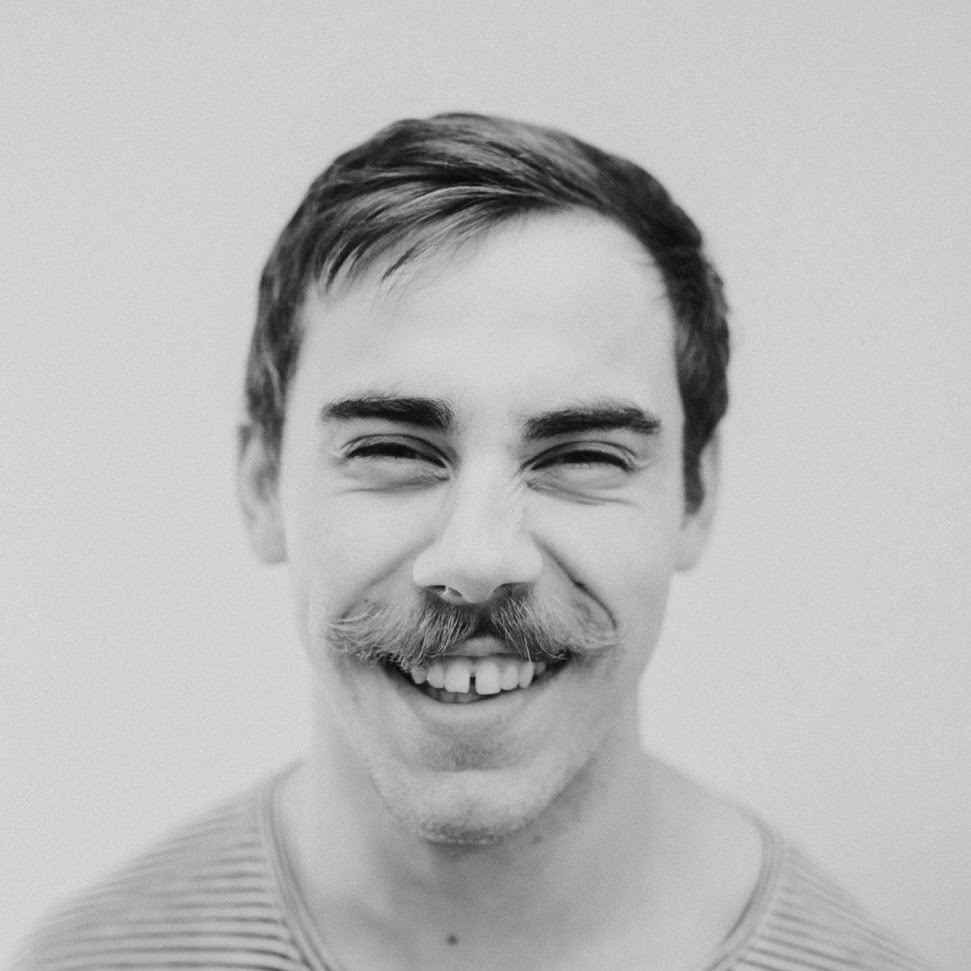
\includegraphics[width=0.7\textwidth]{figures/isak.jpg}
            \end{figure}
        \end{column}
    \end{columns}
\end{frame}


\begin{frame}{Importance and Motivation of the Cahn Hilliard Equation}
    \begin{columns}
        % Column 1
        \begin{column}{0.5\textwidth}
            \begin{itemize}
                \item Thermodynamically modelling of a two-component liquid separation.
                \item Droplet dynamics, i.e., coalescence, breakup and movement by coupling with Navier-Stokes.
            \end{itemize}
        \end{column}
        % Column 1
        \begin{column}{0.5\textwidth}
            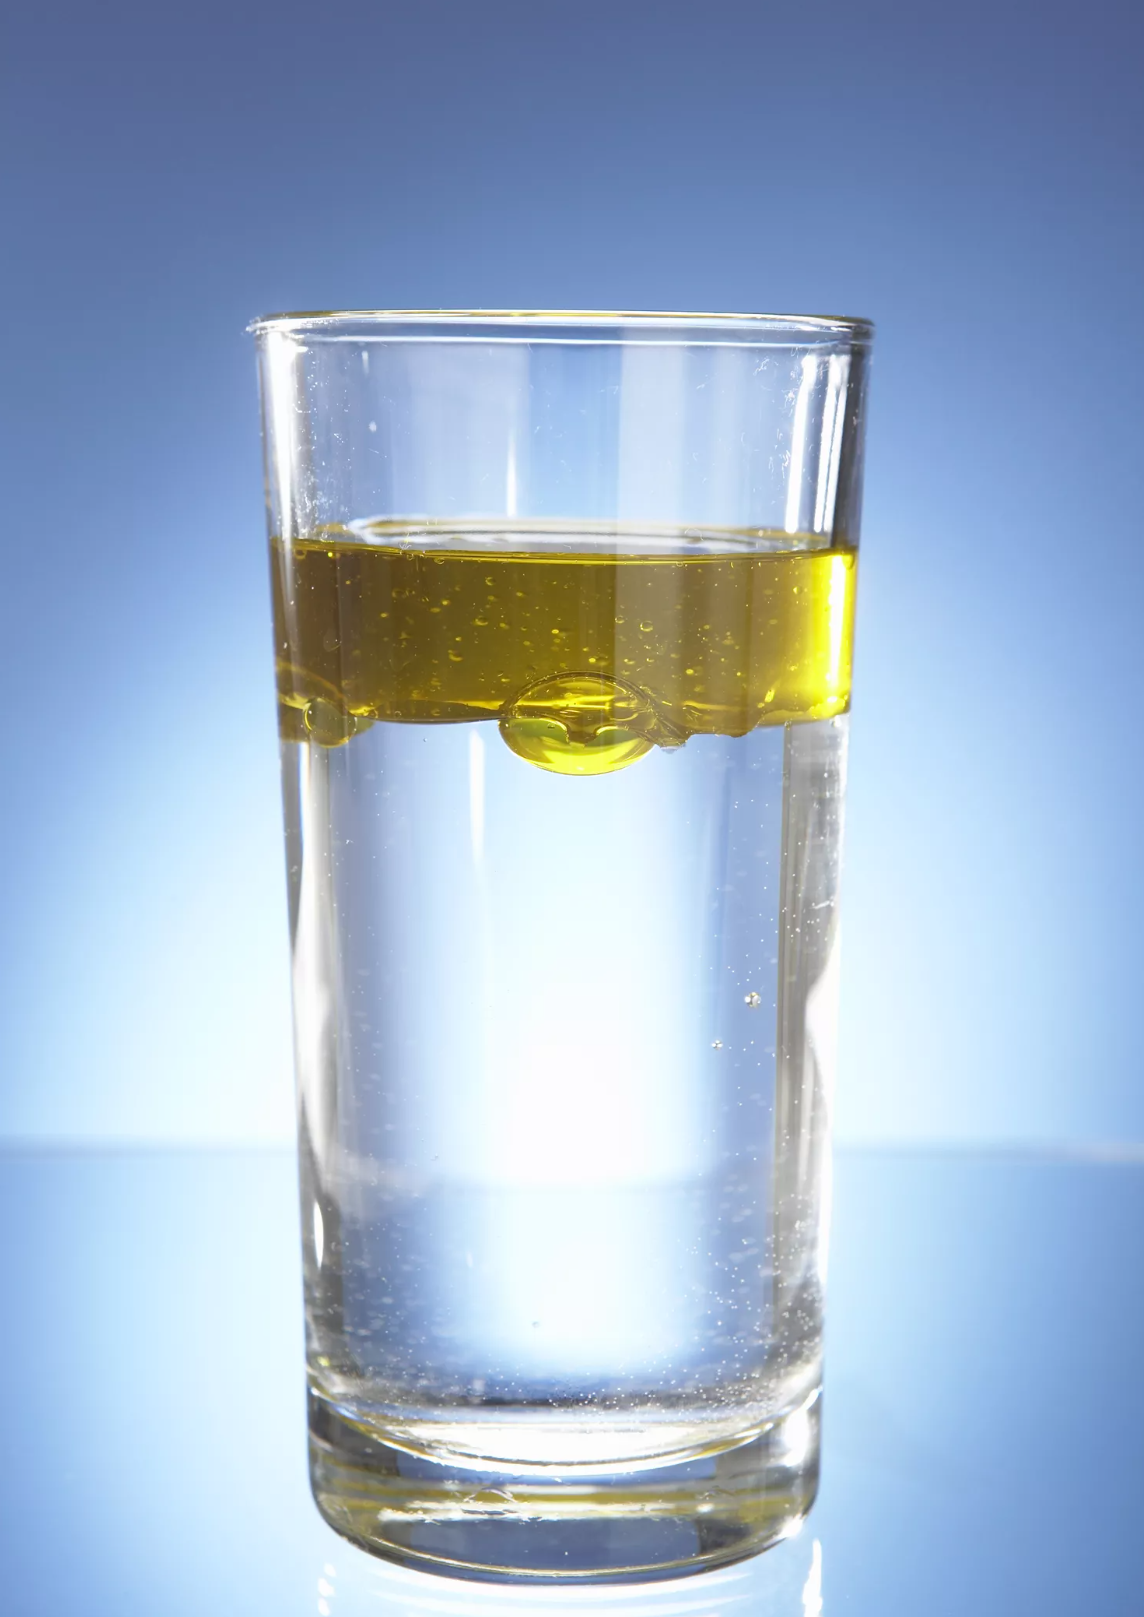
\includegraphics[width=0.5\textwidth]{CH-example/oil1.png}
        \end{column}
    \end{columns}
\end{frame}

\begin{frame}{Importance and Motivation of the Cahn Hilliard Equation}
    \begin{columns}
        % Column 1
        \begin{column}{0.5\textwidth}
            \begin{itemize}
            \item Modelling of so-called lipid rafts in biological membrane dynamics.
            \end{itemize}
        \end{column}
        % Column 1
        \begin{column}{0.9\textwidth}
            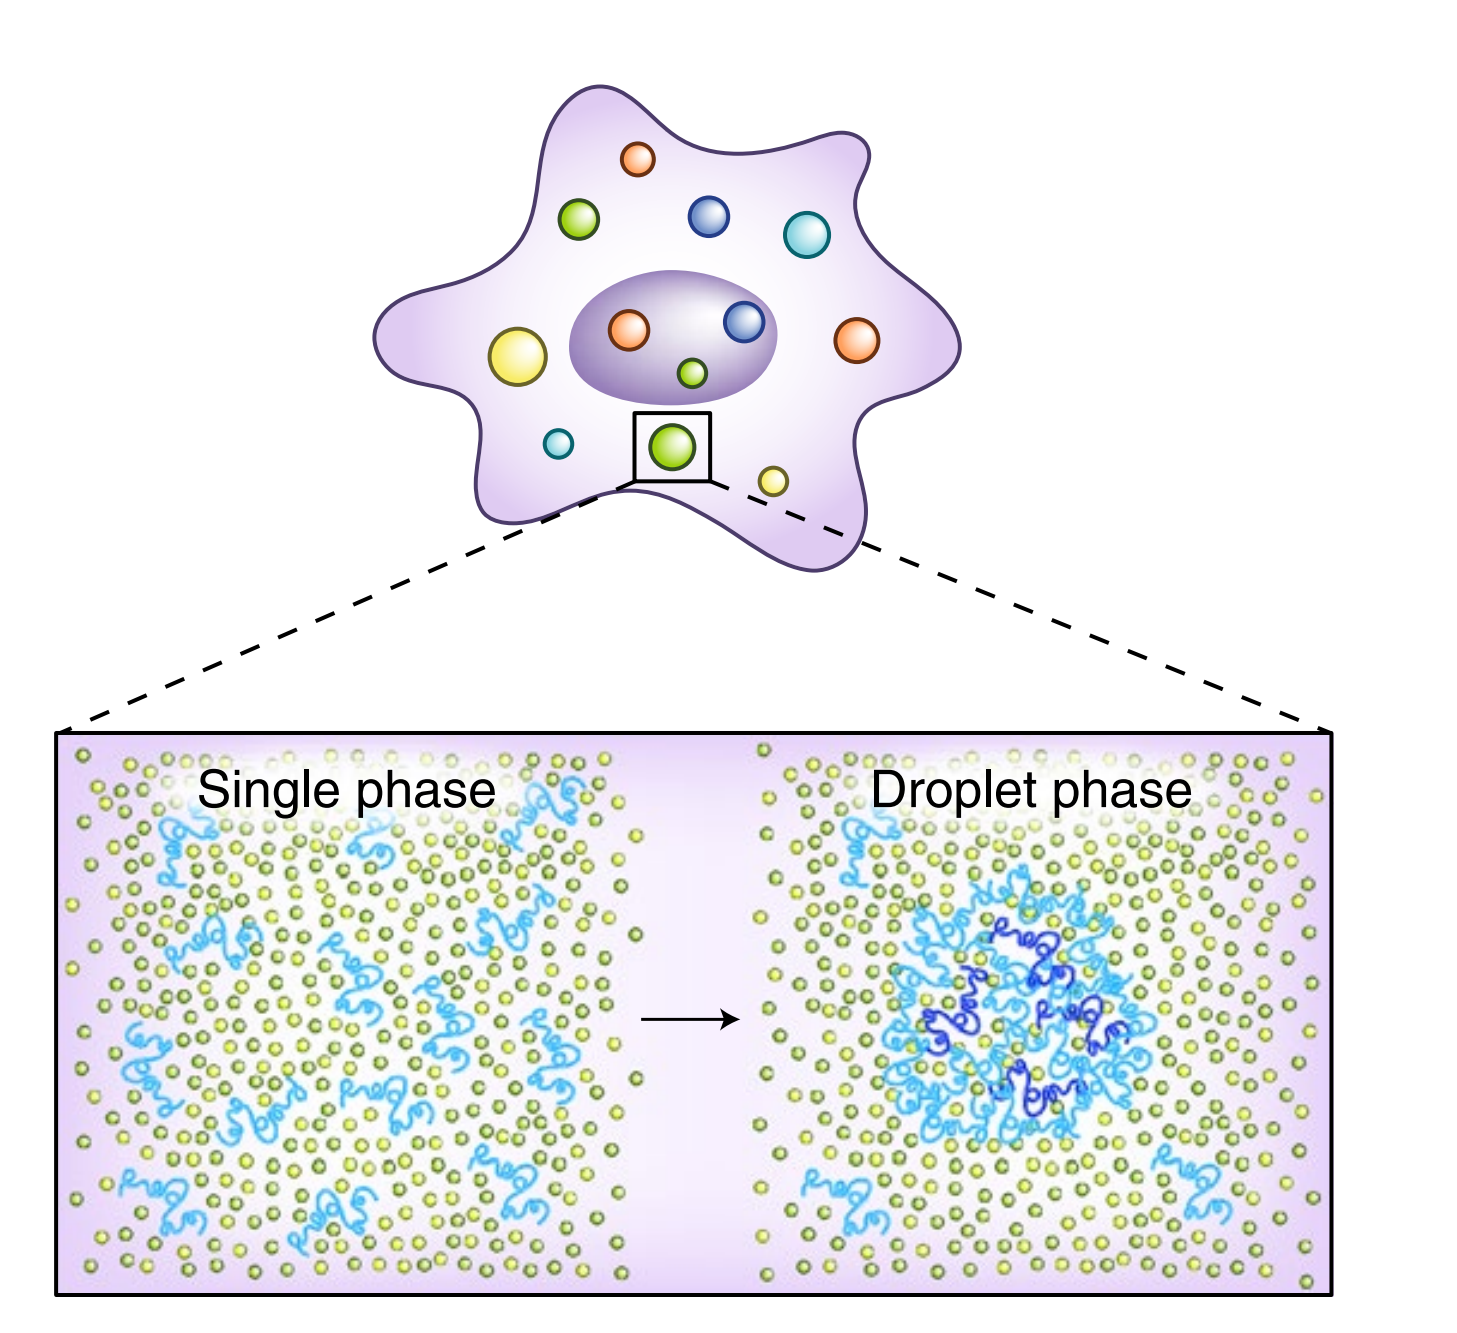
\includegraphics[width=0.5\textwidth]{CH-example/oil2.png}
        \end{column}
    \end{columns}
\end{frame}


\begin{frame}
    \begin{block}{The Cahn Hilliard Equation}
        The general Cahn Hilliard Equation  has the form $u( x, t): \Omega \times [0,T] \mapsto [-1,1]   $ s.t.
            \[
            \begin{split}
                 u_t+\Delta\left(\varepsilon^2 \Delta u- f(u)\right)&=0 \quad \text{in } \Omega \\
\partial_n u=\partial_n \Delta u& =0 \quad \text{on } \Gamma  \\
 u & =u_0 \quad \text{on } \Omega
            \end{split}
            \]
where $f(s)=F^{\prime}(s)$, where we define the chemical energy $F(s)=\frac{1}{4}\left(s^2-1\right)^2$,  $\Omega \subset \mathbf{R}^d$, is a bounded domain.
\end{block}
\begin{block}{Challenges}
    \begin{enumerate}
        \item Highly nonlinear and stiff. $\implies \text{IMEX method} $.
            % \item 4th order system. \text{Solved using a FEM method} $
    \end{enumerate}
\end{block}
\end{frame}

\begin{frame}
    \begin{block}{Why Finite Element Method (FEM)}
        \begin{enumerate}
            \item \textbf{Robust mathematical framework}
            \item \textbf{Can easily handle complex geometries}
            \item \textbf{High flexibility of basis functions}
            \item \textbf{Other: } Supports adaptive refinements, easily adaptable to multi-physics problems ++ .
        \end{enumerate}
    \end{block}
\end{frame}


\begin{frame}
    \frametitle{The Biharmonic Problem (on a polygon)}
    \begin{columns}
        \column{0.55\textwidth}
        \begin{block}{}
            Let $\Omega \approx \Omega_{h} = \mathcal{T}_{h}$ be a bounded \textcolor{red}{polygonal} domain with boundary $\Gamma $ . Let the biharmonic problem have the form s.t. $u:\Omega \mapsto \mathbb{R} $,
            \begin{equation}
                \label{eq:bi_problem}
                \begin{split}
                    \Delta^2 u + \alpha u & = f( x) \quad \text{in } \Omega, \\
                    \partial_{n} u & = 0 \quad \text{on } \Gamma , \\
                    \partial_{n} \Delta u & = 0 \quad \text{on } \Gamma . \\
                \end{split}
            \end{equation}
            Here is $\Delta ^2 = \Delta \left( \Delta \right) $ the biharmonic operator.
        \end{block}

        \column{0.45\textwidth}
        \begin{figure}[htpb!]
            \centering
            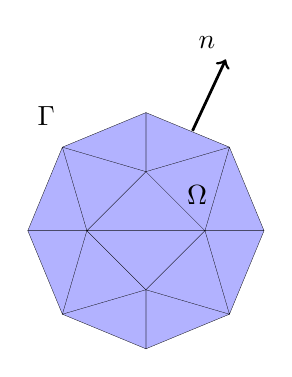
\begin{tikzpicture}
                % FIGURE OF FITTED MESH
                % Boundary points
                \foreach \i in {0, 45, ..., 315} {
                    \coordinate (boundary-\i) at (\i:1.5cm);
                }
                % Interior points
                \coordinate (interior-1) at (0.75, 0);
                \coordinate (interior-2) at (-0.75, 0);
                \coordinate (interior-3) at (0, 0.75);
                \coordinate (interior-4) at (0, -0.75);

                % Create a cycle connecting all the boundary points
                \fill[blue!30] (boundary-0) -- (boundary-45) -- (boundary-90) -- (boundary-135) -- (boundary-180) -- (boundary-225) -- (boundary-270) -- (boundary-315) -- cycle;

                % Labels
                \node[below right] at (0.4,0.7) {$\Omega $};
                \node[below right] at (-1.5,1.7) {$\Gamma $};

                % Triangulation (manually specified)
                \draw[line width=0.1pt] (boundary-0) -- (boundary-45) -- (interior-1) -- cycle;
                \draw[line width=0.1pt] (boundary-45) -- (boundary-90) -- (interior-3) -- cycle;
                \draw[line width=0.1pt] (boundary-90) -- (boundary-135) -- (interior-3) -- cycle;
                \draw[line width=0.1pt] (boundary-135) -- (boundary-180) -- (interior-2) -- cycle;
                \draw[line width=0.1pt] (boundary-180) -- (boundary-225) -- (interior-2) -- cycle;
                \draw[line width=0.1pt] (boundary-225) -- (boundary-270) -- (interior-4) -- cycle;
                \draw[line width=0.1pt] (boundary-270) -- (boundary-315) -- (interior-4) -- cycle;
                \draw[line width=0.1pt] (boundary-315) -- (boundary-0) -- (interior-1) -- cycle;

                % Triangulation between interior points
                \draw[line width=0.1pt] (interior-1) -- (interior-2) -- (interior-3) -- cycle;
                \draw[line width=0.1pt] (interior-1) -- (interior-2) -- (interior-4) -- cycle;

                \draw[->, line width=1.0pt] ({1.4*cos(65)}, { 1.4*sin(65) }) -- ({ 2.4*cos(65)  }, { 2.4*sin(65)  }) node[ above left] {$n $};

            \end{tikzpicture}
            \caption{ Illustration of the mesh $\Omega_{h} $, the boundary $\Gamma $ and the normal vector $n$. }
            \label{fig:domain_construction}
        \end{figure}
    \end{columns}
\end{frame}



\begin{frame}
\frametitle{ $C^0$ Interior Penalty Method (CIP) for the Biharmonic Problem }

\begin{block}{}
The proposed numerical scheme is to find an  $w \in V_{h}$ .t.
\begin{equation*}
a_{h}( w, v )   = l_{h}( v) = ( f,v)_{\Omega } , \quad \forall v \in V_{h}  .
\end{equation*}
where
\begin{equation*}
\begin{split}
a_{h} \left( w, v \right)   =&
    \left( \alpha  w, v \right) _{\Omega }   +  \left( \Delta  w, \Delta v \right) _{\Omega } \\
 & +
  \left( \mean{  \Delta  w }, \jump{ \partial _{n }v} \right)_{\mathcal{F}_{h}}  +
 \left( \mean{ \Delta  v }, \jump{ \partial _{n}w }      \right)_{\mathcal{F}_{h}}  + \frac{\gamma }{h}  \left( \jump{ \partial _{n} w}, \jump{ \partial _{n} v   }   \right)_{\mathcal{F}_{h}}
 % l_{h}( v_{h}) & =  \left( f, v \right) _{\Omega }
\end{split}
\end{equation*}

Which is inspired from Brenner2012 \footnotemark[1]
\end{block}

\footnotetext[1]{\fullcite{brenner2012}}

\end{frame}


\begin{frame}
\frametitle{Cut Finite Element Method (CutFEM)}

\begin{block}{Unfitted mesh vs fitted mesh}
    CutFEM is a numerical method for solving partial differential equations (PDEs) using an unfitted mesh.

\begin{figure}
    \centering
    % First TikZ picture
    \begin{minipage}{0.45\textwidth}
        \centering
        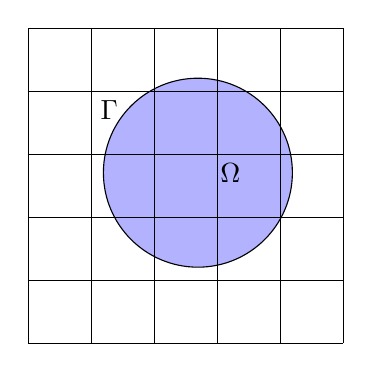
\begin{tikzpicture}[scale=0.80]
            \draw[fill=blue!30] (0.2, 0.2) circle (1.5cm);
            % Background mesh
            \foreach \i in {-2.5, -1.5, ..., 2.5} {
                \draw[line width=0.1pt, shift={(-2.5,\i)}] (0,0) -- (5,0);
                \draw[line width=0.1pt, shift={(\i,-2.5)}] (0,0) -- (0,5);
            }
            % Labels
            \node[below right] at (0.4,0.5) {$\Omega $};
            \node[below right] at (-1.5,1.5) {$\Gamma $};
            % \draw[blue, thick] (-2.5, -2.5) rectangle (2.5, 2.5);
        \end{tikzpicture}
    \end{minipage}
    \hfill
    % Second TikZ picture
    \begin{minipage}{0.45\textwidth}
        \centering
        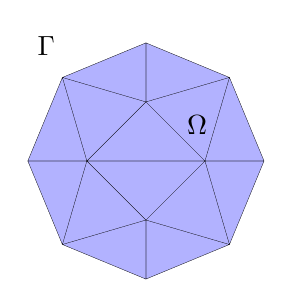
\begin{tikzpicture}[scale=1.0]
            % FIGURE OF UNFITTED MESH
            % Boundary points
            \foreach \i in {0, 45, ..., 315} {
                \coordinate (boundary-\i) at (\i:1.5cm);
            }
            % Interior points
            \coordinate (interior-1) at (0.75, 0);
            \coordinate (interior-2) at (-0.75, 0);
            \coordinate (interior-3) at (0, 0.75);
            \coordinate (interior-4) at (0, -0.75);

            % Create a cycle connecting all the boundary points
            \fill[blue!30] (boundary-0) -- (boundary-45) -- (boundary-90) -- (boundary-135) -- (boundary-180) -- (boundary-225) -- (boundary-270) -- (boundary-315) -- cycle;

            % Labels
            \node[below right] at (0.4,0.7) {$\Omega $};
            \node[below right] at (-1.5,1.7) {$\Gamma $};

            % Triangulation (manually specified)
            \draw[line width=0.1pt] (boundary-0) -- (boundary-45) -- (interior-1) -- cycle;
            \draw[line width=0.1pt] (boundary-45) -- (boundary-90) -- (interior-3) -- cycle;
            \draw[line width=0.1pt] (boundary-90) -- (boundary-135) -- (interior-3) -- cycle;
            \draw[line width=0.1pt] (boundary-135) -- (boundary-180) -- (interior-2) -- cycle;
            \draw[line width=0.1pt] (boundary-180) -- (boundary-225) -- (interior-2) -- cycle;
            \draw[line width=0.1pt] (boundary-225) -- (boundary-270) -- (interior-4) -- cycle;
            \draw[line width=0.1pt] (boundary-270) -- (boundary-315) -- (interior-4) -- cycle;
            \draw[line width=0.1pt] (boundary-315) -- (boundary-0) -- (interior-1) -- cycle;

            % Triangulation between interior points
            \draw[line width=0.1pt] (interior-1) -- (interior-2) -- (interior-3) -- cycle;
            \draw[line width=0.1pt] (interior-1) -- (interior-2) -- (interior-4) -- cycle;

            % \draw[blue, thick] (-2.5, -2.5) rectangle (2.5, 2.5);

        \end{tikzpicture}
    \end{minipage}


    % \caption{Mesh comparison: unfitted mesh (left) adheres to domain and boundary, while fitted mesh (right) employs a triangular mesh for polygonal approximation of the circular domain.}
    \label{fig:domain_mesh}
    \end{figure}
\end{block}

\end{frame}

\begin{frame}
    \frametitle{Cut Finite Element Method}
Background Mesh
    \begin{block}{}
        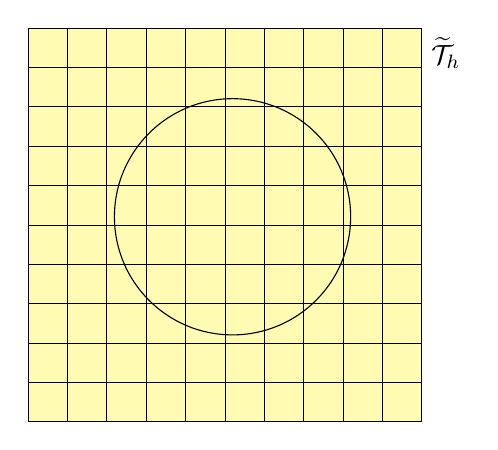
\begin{tikzpicture}[scale=1.0]

            \fill[yellow!30] (-2.5,2.5) -- (2.5,2.5) -- (2.5,-2.5) -- (-2.5,-2.5) -- cycle;

            \draw (0.1, 0.1) circle (1.5cm);
            % Background mesh
            \foreach \i in {-2.5, -2, ..., 2.5} {
                \draw[line width=0.1pt, shift={(-2.5,\i)}] (0,0) -- (5,0);
                \draw[line width=0.1pt, shift={(\i,-2.5)}] (0,0) -- (0,5);
            }


            % Labels
            \node[below right] at (2.5,2.5) {$\widetilde{\mathcal{T}}_{h}$};
        \end{tikzpicture}
    \end{block}
\end{frame}

\begin{frame}
    \frametitle{Cut Finite Element Method}
    Active Mesh
    \begin{block}{}
        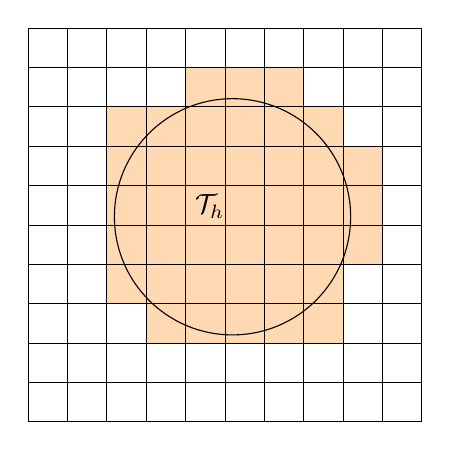
\begin{tikzpicture}[scale=1.0]

            % POTENTIAL ACTIVE MESH
            \fill[orange!30] (2,2) -- (2,-1.5) --(-1.5,-1.5) -- (-1.5,2) -- cycle;

            % ELEMENTS WITH NO INTERSECTION
            % lower left
            \fill[white] (-1.5,-1.5) rectangle (-1.0,-1.0);
            \fill[white] (-1.5,2.0) rectangle (-1.0,1.5);
            \fill[white] (-1.0,2.0) rectangle (-0.5,1.5);
            \fill[white] (2,2) rectangle (1.5,1.5);
            \fill[white] (1.5,2) rectangle (1.0,1.5);
            \fill[white] (2,1.5) rectangle (1.5,1.0);
            \fill[white] (1.5,-1) rectangle (2,-1.5);
            \fill[white] (1.5,-0.5) rectangle (2,-1.0);

            % CUT ELEMENTS
            \fill[orange!30] (-0.5,2.0) rectangle (1.0,1.5);
            \fill[orange!30] (-1.5,1.5) rectangle (0.0,1.0);
            \fill[orange!30] (0.5,1.5) rectangle (1.5,1.0);
            \fill[orange!30] (-1.5,1.0) rectangle (-1.0,-1.0);
            \fill[orange!30] (-1.0,-0.5) rectangle (-0.5,-1.5);
            \fill[orange!30] (-0.5,-1.5) rectangle (1.5,-1.0);
            \fill[orange!30] (1.5,-1) rectangle (1.0,-0.0);
            \fill[orange!30] (1.5,-0.5) rectangle (2.0,1.0);
            \fill[orange!30] (1.0,0.5) rectangle (1.5,1.0);

            \draw (0.1, 0.1) circle (1.5cm);
            % Background mesh
            \foreach \i in {-2.5, -2, ..., 2.5} {
                \draw[line width=0.1pt, shift={(-2.5,\i)}] (0,0) -- (5,0);
                \draw[line width=0.1pt, shift={(\i,-2.5)}] (0,0) -- (0,5);
            }


            % Labels
            % \node[below right] at (2.5,2.5) {$\widetilde{\mathcal{T}}_{h}$};
            % \node[below right] at (0.4,0.5) {$\mathcal{T}_{int}$};
            \node[below right] at (-0.5,0.5) {$\mathcal{T}_{h }$};
        \end{tikzpicture}
    \end{block}
\end{frame}

\begin{frame}
    \frametitle{Cut Finite Element Method}
    Interior Mesh and Cut Cells
    \begin{block}{}
        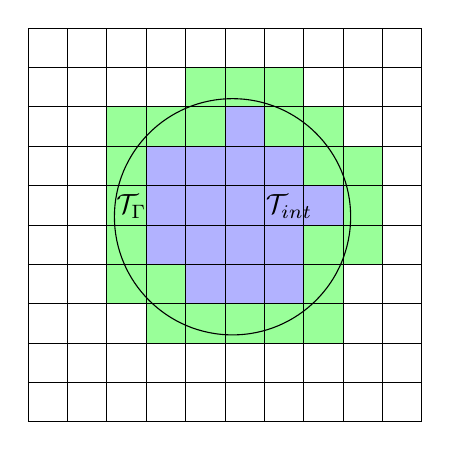
\begin{tikzpicture}[scale=1]

            % POTENTIAL ACTIVE MESH
            \fill[blue!30] (2,2) -- (2,-1.5) --(-1.5,-1.5) -- (-1.5,2) -- cycle;

            % ELEMENTS WITH NO INTERSECTION
            % lower left
            \fill[white] (-1.5,-1.5) rectangle (-1.0,-1.0);
            \fill[white] (-1.5,2.0) rectangle (-1.0,1.5);
            \fill[white] (-1.0,2.0) rectangle (-0.5,1.5);
            \fill[white] (2,2) rectangle (1.5,1.5);
            \fill[white] (1.5,2) rectangle (1.0,1.5);
            \fill[white] (2,1.5) rectangle (1.5,1.0);
            \fill[white] (1.5,-1) rectangle (2,-1.5);
            \fill[white] (1.5,-0.5) rectangle (2,-1.0);

            % CUT ELEMENTS
            \fill[green!40] (-0.5,2.0) rectangle (1.0,1.5);
            \fill[green!40] (-1.5,1.5) rectangle (0.0,1.0);
            \fill[green!40] (0.5,1.5) rectangle (1.5,1.0);
            \fill[green!40] (-1.5,1.0) rectangle (-1.0,-1.0);
            \fill[green!40] (-1.0,-0.5) rectangle (-0.5,-1.5);
            \fill[green!40] (-0.5,-1.5) rectangle (1.5,-1.0);
            \fill[green!40] (1.5,-1) rectangle (1.0,-0.0);
            \fill[green!40] (1.5,-0.5) rectangle (2.0,1.0);
            \fill[green!40] (1.0,0.5) rectangle (1.5,1.0);

            \draw (0.1, 0.1) circle (1.5cm);
            % Background mesh
            \foreach \i in {-2.5, -2, ..., 2.5} {
                \draw[line width=0.1pt, shift={(-2.5,\i)}] (0,0) -- (5,0);
                \draw[line width=0.1pt, shift={(\i,-2.5)}] (0,0) -- (0,5);
            }


            % Labels
            \node[below right] at (0.4,0.5) {$\mathcal{T}_{int}$};
            \node[below right] at (-1.5,0.5) {$\mathcal{T}_{\Gamma }$};
        \end{tikzpicture}
    \end{block}
\end{frame}

\begin{frame}
\frametitle{Cut Finite Element Method}

A recent and promising numerical technique for PDEs, has gained significant momentum in the past decade \footnotemark[1]\footnotemark[2].

\begin{block}{}
    \begin{itemize}
        \item  Complex domains and moving domains efficiently.
        \item Utilizing so-called ghost penalties to ensure well-posedness.
        % \item Dividing the computational domains into \textbf{background} , \textbf{active}, \textbf{cut}  and \textbf{interior} mesh.
    \end{itemize}
\end{block}
\footnotetext[1]{\fullcite{burman2015cutfem}}
\footnotetext[2]{\fullcite{gurkan2019stabilized}}

\end{frame}


\begin{frame}
\frametitle{ Cut $C^0$ Interior Penalty Method (CutCIP) }

\begin{block}{}
The discretized numerical problem is to solve $w \in V_{h}$ such that
\begin{equation*}
A( w, v )  = a_{h}( w,v) + \textcolor{red}{g_{h}( w,v)}  = l_{h}( v), \quad \forall v \in V_{h}  .
\end{equation*}

Where the additional bilinear term $g_{h}( w,v) : V_{h} \times V_{h} \to  \mathbb{R} $ is the so-called \textbf{ghost penalty}, which does the numerical regularization to ensure stability on cut cells.

\end{block}

\end{frame}

\begin{frame}
\frametitle{ Cut $C^0$ Interior Penalty Method}

My master's thesis is dedicated to demonstrating that the relevant properties remain valid for CutCIP formulation still holds.

%     \begin{block}{Well-posedness }
%          The discrete bilinear form $a_{h}$ is wellposed on $V_{h}$ if this holds; \[
%              \begin{split}
%                  (Coercivity) \quad  A( v,v) &  \gtrsim  \| v \|_{A }^{ 2 } \quad  \forall v \in  V_{h} \\
%             (Boundedness) \quad A( v,w) & \lesssim  \| v \|_{A }^{  }\| w \|_{a_{h} }^{  } \quad  \forall v,w \in  V_{h}
%              \end{split}
%         \]
%     \end{block}

    \begin{block}{A Priori Estimates }

         Let $u$ be the solution to the strong problem with the corresponding discrete solution $u_{h}$ with polynomical order $k\ge 2$ .
        Then does it exist  $l = \min_{} ( 2, k)  $ s.t.
\[
        \| u - u_{h} \|_{a_{h}  }^{  } \lesssim  h^{l-1} \| u \|_{ H^{l} ( \Omega ) }^{  }
\]
    \end{block}
    \footnotetext[1]{\fullcite{Gu2012}}
\end{frame}



\begin{frame}
\frametitle{ Cut $C^0$ Interior Penalty Method Results }
% \frametitle{Manufactured Solution}


\begin{block}{Manufactured solution}
    In the experiments will we only consider polynomial order $k=2$.
We consider the manufactured solution:
$$
u_{ex}(\mathbf{x}) = \left(x_1^2 + x_2^2 - 1\right)^2 \cos(2\pi x_1) \cos(2\pi x_2)
$$
where $\mathbf{x}=(x_1,x_2)$ and $\Omega=\{(x_1,x_2): x_1^2 + x_2^2 \le  1\}$.
This manufactured solution can be used to test the accuracy of numerical methods for solving the above differential equation.
\end{block}
\end{frame}


\begin{frame}
\frametitle{ Cut $C^0$ Interior penalty method (CutCIP) Results }
\resizebox{\textwidth}{!}{
\begin{tabular}{rrrrrrrrr}
    \hline\hline
    \textbf{$n$} & \textbf{$\Vert e \Vert_{L^2}$} & \textbf{EOC} & \textbf{$ \Vert e \Vert_{H^1}$} & \textbf{EOC} & \textbf{$\Vert e \Vert_{ a_h,* }$} & \textbf{EOC} & \textbf{Cond number} & \textbf{ndofs} \\\hline
    4 & 2.4E+00 &  & 3.3E+00 &  & 6.2E+01 &  & 8.7E+04 & 8.1E+01 \\
    8 & 3.6E-01 & 2.72 & 1.1E+00 & 1.60 & 3.9E+01 & 0.68 & 5.1E+05 & 2.4E+02 \\
    16 & 2.2E-02 & 4.06 & 2.5E-01 & 2.12 & 1.4E+01 & 1.51 & 3.7E+06 & 8.3E+02 \\
    32 & 5.6E-03 & 1.97 & 6.0E-02 & 2.04 & 3.6E+00 & 1.93 & 2.8E+07 & 3.0E+03 \\
    64 & 1.4E-03 & 2.00 & 1.5E-02 & 2.02 & 9.2E-01 & 1.96 & 2.1E+08 & 1.1E+04 \\
    128 & 3.5E-04 & 2.00 & 3.7E-03 & 2.01 & 2.4E-01 & 1.94 & 1.7E+09 & 4.3E+04 \\\hline\hline
  \end{tabular}
}
\end{frame}






\begin{frame}
\frametitle{ Cut $C^0$ Interior penalty method (CutCIP) Results }

\begin{figure}[h!]
    \centering
    \resizebox{0.6\textwidth}{!}{% Recommended preamble:
% \usetikzlibrary{arrows.meta}
% \usetikzlibrary{backgrounds}
% \usepgfplotslibrary{patchplots}
% \usepgfplotslibrary{fillbetween}
% \pgfplotsset{%
%     layers/standard/.define layer set={%
%         background,axis background,axis grid,axis ticks,axis lines,axis tick labels,pre main,main,axis descriptions,axis foreground%
%     }{
%         grid style={/pgfplots/on layer=axis grid},%
%         tick style={/pgfplots/on layer=axis ticks},%
%         axis line style={/pgfplots/on layer=axis lines},%
%         label style={/pgfplots/on layer=axis descriptions},%
%         legend style={/pgfplots/on layer=axis descriptions},%
%         title style={/pgfplots/on layer=axis descriptions},%
%         colorbar style={/pgfplots/on layer=axis descriptions},%
%         ticklabel style={/pgfplots/on layer=axis tick labels},%
%         axis background@ style={/pgfplots/on layer=axis background},%
%         3d box foreground style={/pgfplots/on layer=axis foreground},%
%     },
% }

\begin{tikzpicture}[/tikz/background rectangle/.style={fill={rgb,1:red,1.0;green,1.0;blue,1.0}, fill opacity={1.0}, draw opacity={1.0}}, show background rectangle]
\begin{axis}[point meta max={nan}, point meta min={nan}, legend cell align={left}, legend columns={1}, title={}, title style={at={{(0.5,1)}}, anchor={south}, font={{\fontsize{14 pt}{18.2 pt}\selectfont}}, color={rgb,1:red,0.0;green,0.0;blue,0.0}, draw opacity={1.0}, rotate={0.0}, align={center}}, legend style={color={rgb,1:red,0.0;green,0.0;blue,0.0}, draw opacity={1.0}, line width={1}, solid, fill={rgb,1:red,1.0;green,1.0;blue,1.0}, fill opacity={1.0}, text opacity={1.0}, font={{\fontsize{8 pt}{10.4 pt}\selectfont}}, text={rgb,1:red,0.0;green,0.0;blue,0.0}, cells={anchor={center}}, at={(1.02, 1)}, anchor={north west}}, axis background/.style={fill={rgb,1:red,1.0;green,1.0;blue,1.0}, opacity={1.0}}, anchor={north west}, xshift={1.0mm}, yshift={-1.0mm}, width={94.6mm}, height={74.2mm}, scaled x ticks={false}, xlabel={$\delta$}, x tick style={color={rgb,1:red,0.0;green,0.0;blue,0.0}, opacity={1.0}}, x tick label style={color={rgb,1:red,0.0;green,0.0;blue,0.0}, opacity={1.0}, rotate={0}}, xlabel style={at={(ticklabel cs:0.5)}, anchor=near ticklabel, at={{(ticklabel cs:0.5)}}, anchor={near ticklabel}, font={{\fontsize{11 pt}{14.3 pt}\selectfont}}, color={rgb,1:red,0.0;green,0.0;blue,0.0}, draw opacity={1.0}, rotate={0.0}}, xmajorgrids={true}, xmin={-0.001471665988344504}, xmax={0.05052719893316125}, xticklabels={{$0.00$,$0.01$,$0.02$,$0.03$,$0.04$,$0.05$}}, xtick={{0.0,0.010000000000000002,0.020000000000000004,0.030000000000000006,0.04000000000000001,0.05000000000000001}}, xtick align={inside}, xticklabel style={font={{\fontsize{8 pt}{10.4 pt}\selectfont}}, color={rgb,1:red,0.0;green,0.0;blue,0.0}, draw opacity={1.0}, rotate={0.0}}, x grid style={color={rgb,1:red,0.0;green,0.0;blue,0.0}, draw opacity={0.1}, line width={0.5}, solid}, axis x line*={left}, x axis line style={color={rgb,1:red,0.0;green,0.0;blue,0.0}, draw opacity={1.0}, line width={1}, solid}, scaled y ticks={false}, ylabel={$\kappa(A)$}, y tick style={color={rgb,1:red,0.0;green,0.0;blue,0.0}, opacity={1.0}}, y tick label style={color={rgb,1:red,0.0;green,0.0;blue,0.0}, opacity={1.0}, rotate={0}}, ylabel style={at={(ticklabel cs:0.5)}, anchor=near ticklabel, at={{(ticklabel cs:0.5)}}, anchor={near ticklabel}, font={{\fontsize{11 pt}{14.3 pt}\selectfont}}, color={rgb,1:red,0.0;green,0.0;blue,0.0}, draw opacity={1.0}, rotate={0.0}}, ymode={log}, log basis y={10}, ymajorgrids={true}, ymin={100000.0}, ymax={1.0e25}, yticklabels={{$10^{5}$,$10^{10}$,$10^{15}$,$10^{20}$,$10^{25}$}}, ytick={{100000.0,1.0e10,1.0e15,1.0e20,1.0e25}}, ytick align={inside}, yticklabel style={font={{\fontsize{8 pt}{10.4 pt}\selectfont}}, color={rgb,1:red,0.0;green,0.0;blue,0.0}, draw opacity={1.0}, rotate={0.0}}, y grid style={color={rgb,1:red,0.0;green,0.0;blue,0.0}, draw opacity={0.1}, line width={0.5}, solid}, axis y line*={left}, y axis line style={color={rgb,1:red,0.0;green,0.0;blue,0.0}, draw opacity={1.0}, line width={1}, solid}, colorbar={false}]
    [\addlegendimage{empty legend}] \addlegendentry[font={{\fontsize{11 pt}{14.3 pt}\selectfont}}, text={rgb,1:red,0.0;green,0.0;blue,0.0}] {\hspace{-.6cm}{\textbf{$(\gamma, \gamma_1, \gamma_2)$}}}
    \addplot[color={rgb,1:red,0.0;green,0.0;blue,1.0}, name path={e73f70a5-bbbd-4a24-8407-eef9d08bc09d}, draw opacity={1.0}, line width={1}, solid]
        table[row sep={\\}]
        {
            \\
            0.0  1.2679164207221107e8  \\
            0.012263883236204186  1.2718633484176141e8  \\
            0.024527766472408372  1.2693944128424127e8  \\
            0.03679164970861256  1.2718633338545807e8  \\
            0.049055532944816745  1.2679164340263365e8  \\
        }
        ;
    \addlegendentry { $1.0 \cdot 10^{1}$, $0.5 \cdot 10^{1}$, $1.0 \cdot 10^{-1}$ }
    \addplot[color={rgb,1:red,1.0;green,0.0;blue,0.0}, name path={8dbacc37-3690-4b1f-9d5d-1b6f1fc900ac}, draw opacity={1.0}, line width={1}, solid]
        table[row sep={\\}]
        {
            \\
            0.0  4.639960110962716e10  \\
            0.012263883236204186  4.932252358128007e12  \\
            0.024527766472408372  4.0959531093983247e12  \\
            0.03679164970861256  4.932252223523245e12  \\
            0.049055532944816745  4.639960117645048e10  \\
        }
        ;
    \addlegendentry { $1.0 \cdot 10^{1}$, $ 0.0 \cdot 10^{0} $, $ 0.0 \cdot 10^{0} $ }
\end{axis}
\end{tikzpicture}
}
    \caption{The plot presents the $L^2$ and $H^1$ error norms and the error in the energy norm ($\Vert e \Vert_{a_h,*}$).}
    \label{fig:CutFEM_error1}
\end{figure}

\end{frame}

\begin{frame}
\frametitle{The Cahn Hilliard Equation}
    \begin{columns}
        % Left column
        \begin{column}{0.5\textwidth}
            \begin{block}{Recall}
                The problem has the form $u( x, t): \Omega \times [0,T] \mapsto [-1,1]$ s.t.
                \[
                \begin{split}
                    u_t+\Delta\left(\varepsilon \Delta u-\frac{1}{\varepsilon} f(u)\right)&=0 \quad \text{in } \Omega \\
                    \partial_n u=\partial_n \Delta u& =0 \quad \text{on } \Gamma  \\
                    u & =u_0 \quad \text{on } \Omega
                \end{split}
                \]
                where $f(u)$ is a nonlinear function.
            \end{block}
        \end{column}
        % Right column
        \begin{column}{0.5\textwidth}
            \begin{block}{Plan forward}
                \begin{enumerate}
                    \item We have now a tool to solve the $\Delta ( \Delta u) $ operator
                    \item Will utilize the time-iteration scheme to solve non-linearity
                \end{enumerate}
            \end{block}
        \end{column}
    \end{columns}
\end{frame}


\begin{frame}
\frametitle{The CutCIP Cahn-Hilliard Formulation}


Drawing upon the concepts delineated in Feng\footnotemark[1], the most efficient approach to address the nonlinear term is by employing an implicit-explicit (IMEX) scheme.

\begin{block}{IMEX method on the CutCIP formulation}
    Let $u^{m}_{h} \in V_{h}$ for the timesteps $m=0,1,\ldots,M$. Let $u_{h}^{0} = u_{0}$ be the initial timestep, then is.
\[
(\overline{\partial}  _{t} u_{h}^m, v_h ) + \varepsilon A (u_{h}^{m}, v_h )+\frac{1}{\varepsilon} c_h ( u_{h}^{m-1}, v_h)=0 \quad \forall v_h \in V_h^m .
\]
Here is $c_{h}( . , .) $ an the nonlinear terms handled in a implicit fashion. The $ \overline{\partial}  _{t}$ operator is simply a finite difference scheme in time-dimension.

\end{block}

\footnotetext[1]{\fullcite{feng2007fully}}
\end{frame}

\begin{frame}
\frametitle{The CutCIP Cahn-Hilliard Experiments}
Implemented using the Gridap FEM framework written in Julia \footnotemark[1].


\begin{block}{Simulation parameters}
    \begin{itemize}
        \item Physical domain $\Omega$  is a 4 discs of radius $R=1$ with distance $d=0.999$, i.e. they are touching!
        \item Inital data is $u_0 = random(-1,1)$ in physical domain $\Omega $.
        % \item Backgroundmesh with size ($L\times L$ ) for $L=2$ and $n=128$.
        % \item Polynomial order $k=2$ .
        % \item Physical parameter $\varepsilon  = \frac{1}{30}$.
        % \item Time-step $\tau = \varepsilon ^{2} \frac{1}{10} $ for the interval $ 0\le t \le 10^3 \tau $.
    \end{itemize}
\end{block}

\footnotetext[1]{\fullcite{badia2020gridap}}


\end{frame}

% \begin{frame}
% \frametitle{The CutCIP Cahn-Hilliard Experiments}


\begin{frame}
\frametitle{The CutCIP Cahn-Hilliard Experiments}

\begin{figure}[h]
    \centering
    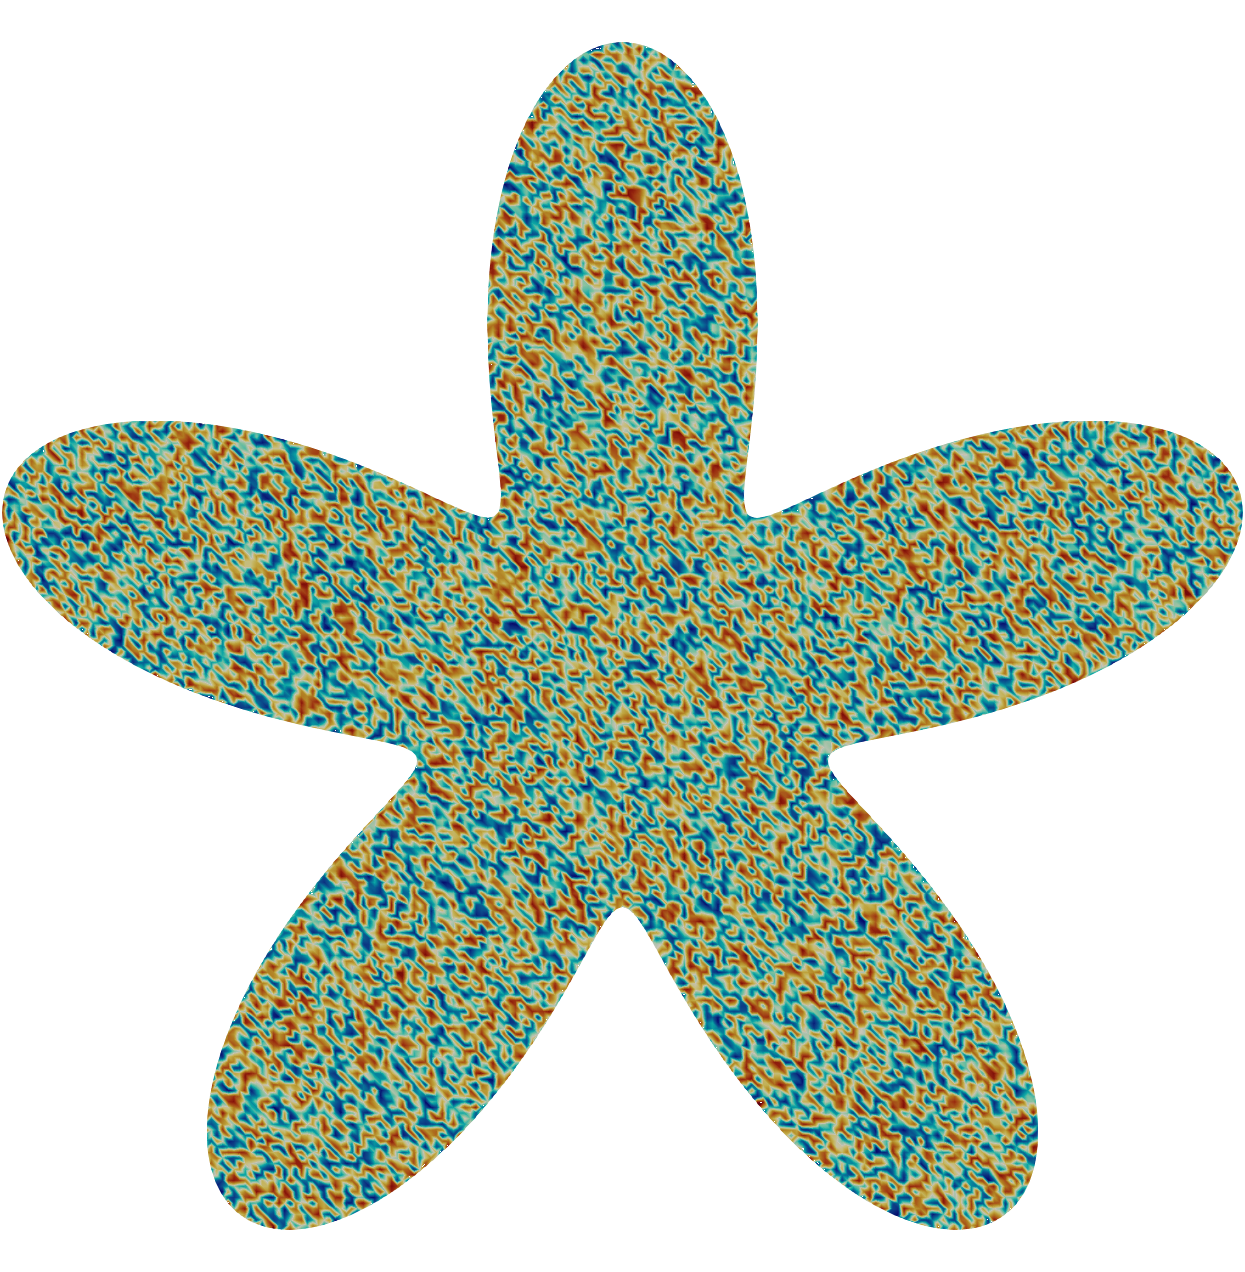
\includegraphics[width=0.5\textwidth]{CH-example/flower_0.png}
    \caption{Iteration 0}
\end{figure}
\end{frame}

\begin{frame}
\frametitle{The CutCIP Cahn-Hilliard Experiments}
\begin{figure}[h]
    \centering
    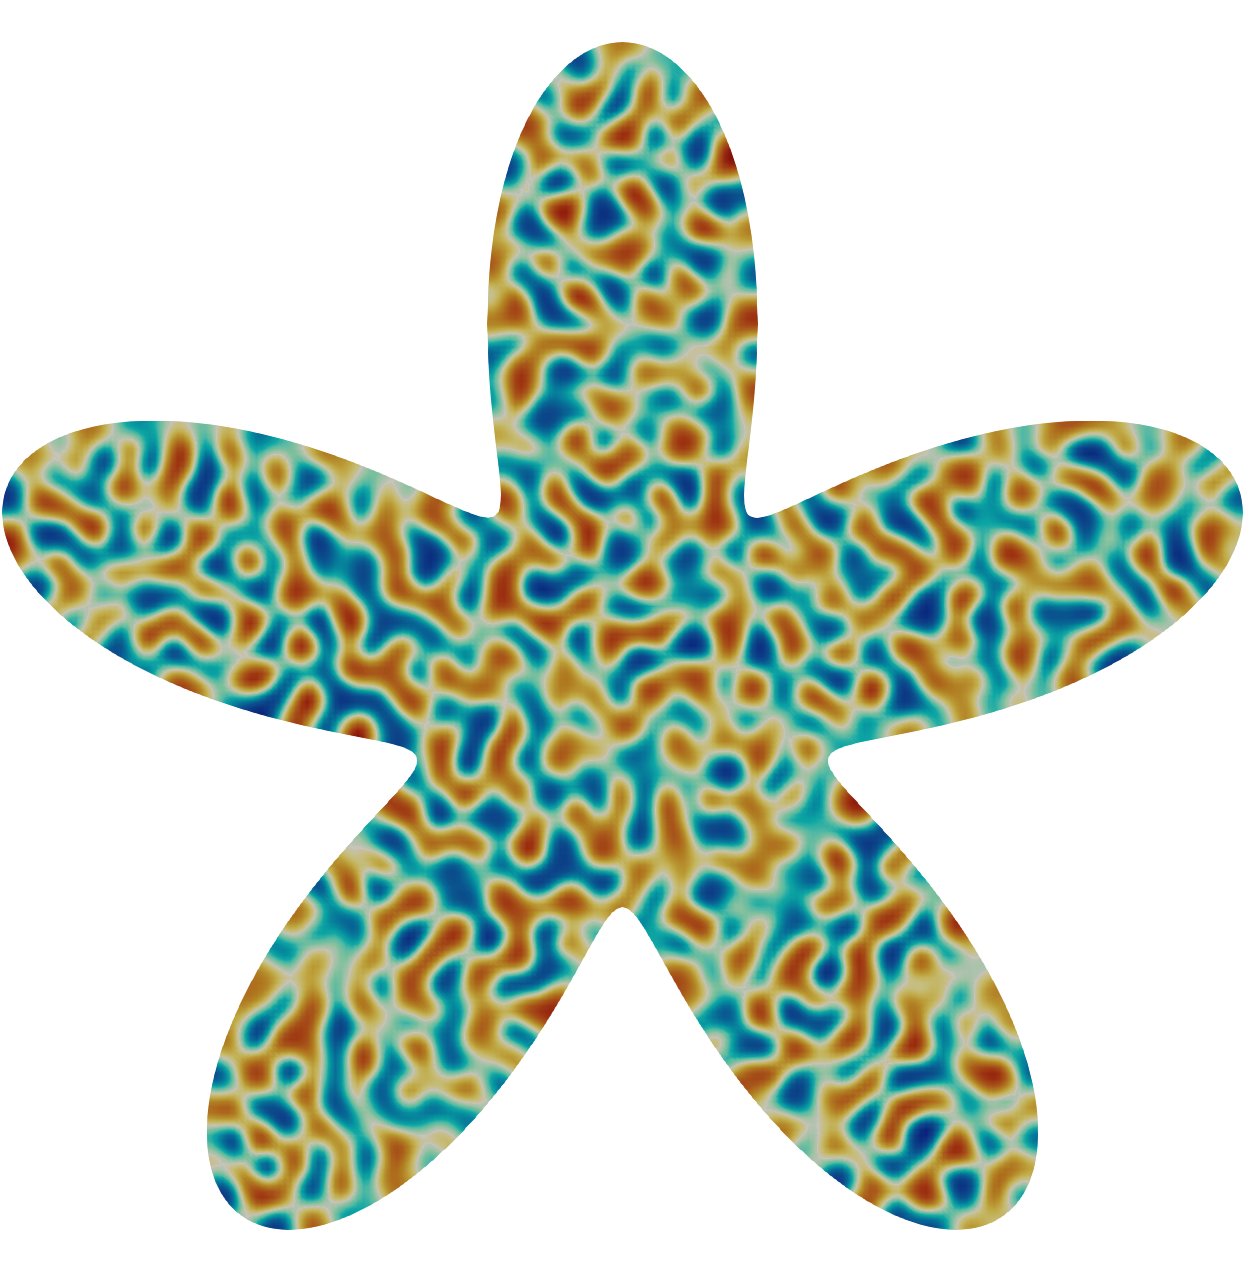
\includegraphics[width=0.5\textwidth]{CH-example/flower_10.png}
    \caption{Iteration 10}
\end{figure}
\end{frame}

\begin{frame}
\frametitle{The CutCIP Cahn-Hilliard Experiments}
\begin{figure}[h]
    \centering
    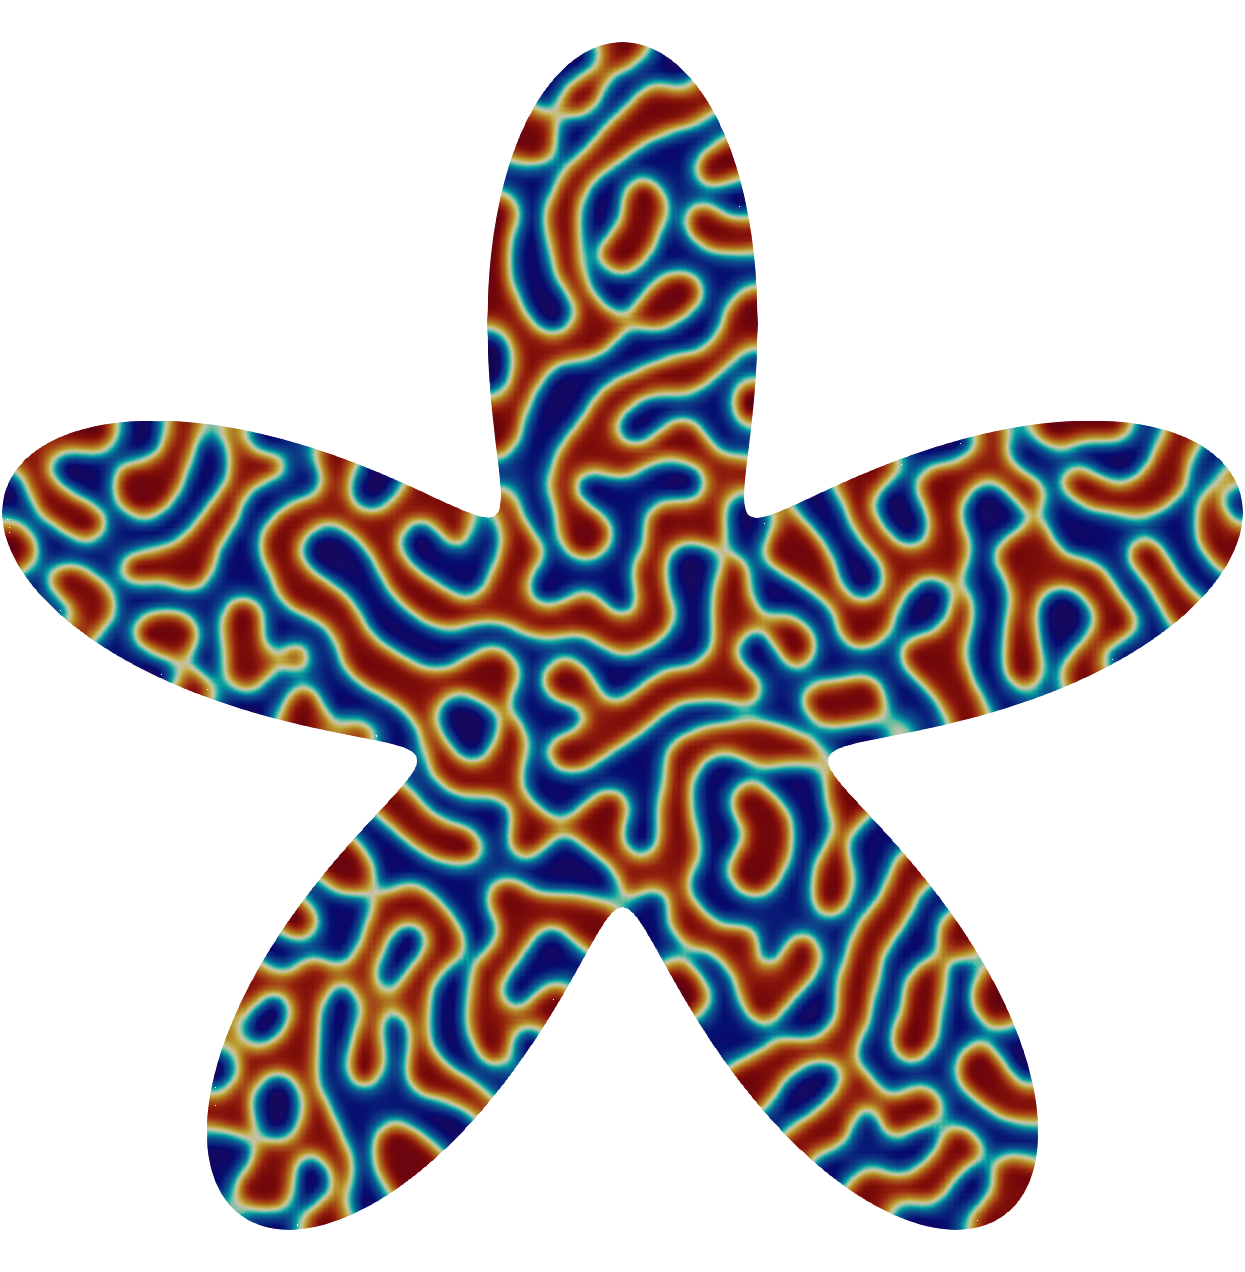
\includegraphics[width=0.5\textwidth]{CH-example/flower_50.png}
    \caption{Iteration 50}
\end{figure}
\end{frame}

\begin{frame}
\frametitle{The CutCIP Cahn-Hilliard Experiments}
\begin{figure}[h]
    \centering
    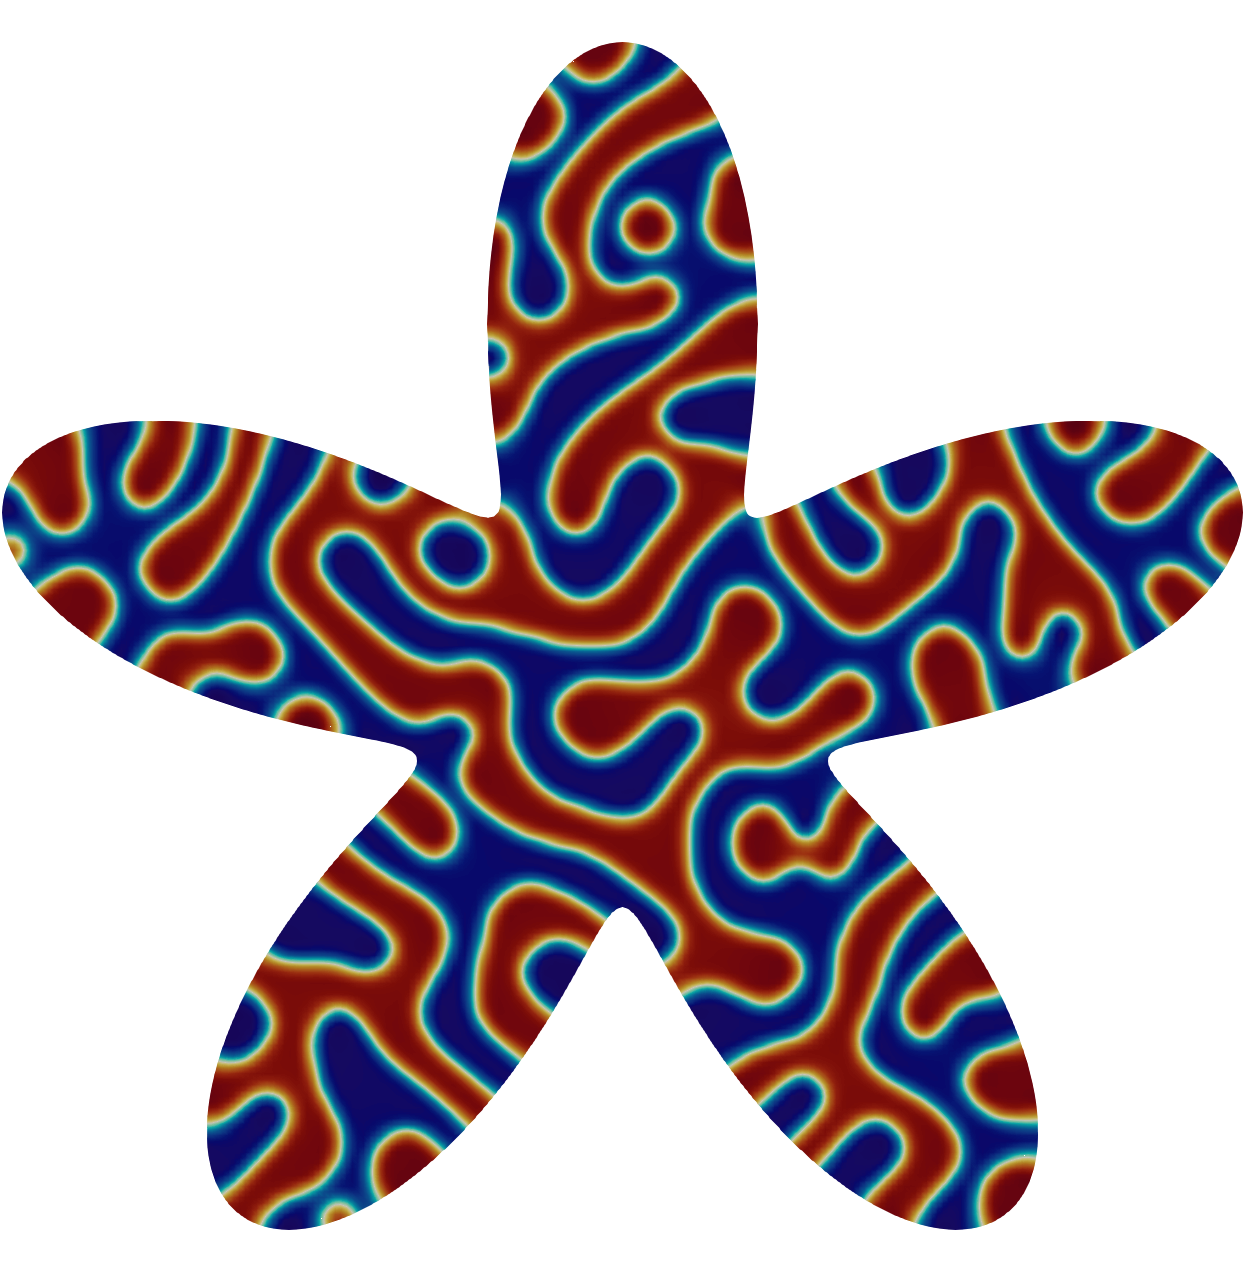
\includegraphics[width=0.5\textwidth]{CH-example/flower_200.png}
    \caption{Iteration 200}
\end{figure}
\end{frame}

\begin{frame}
\frametitle{The CutCIP Cahn-Hilliard Experiments}
\begin{figure}[h]
    \centering
    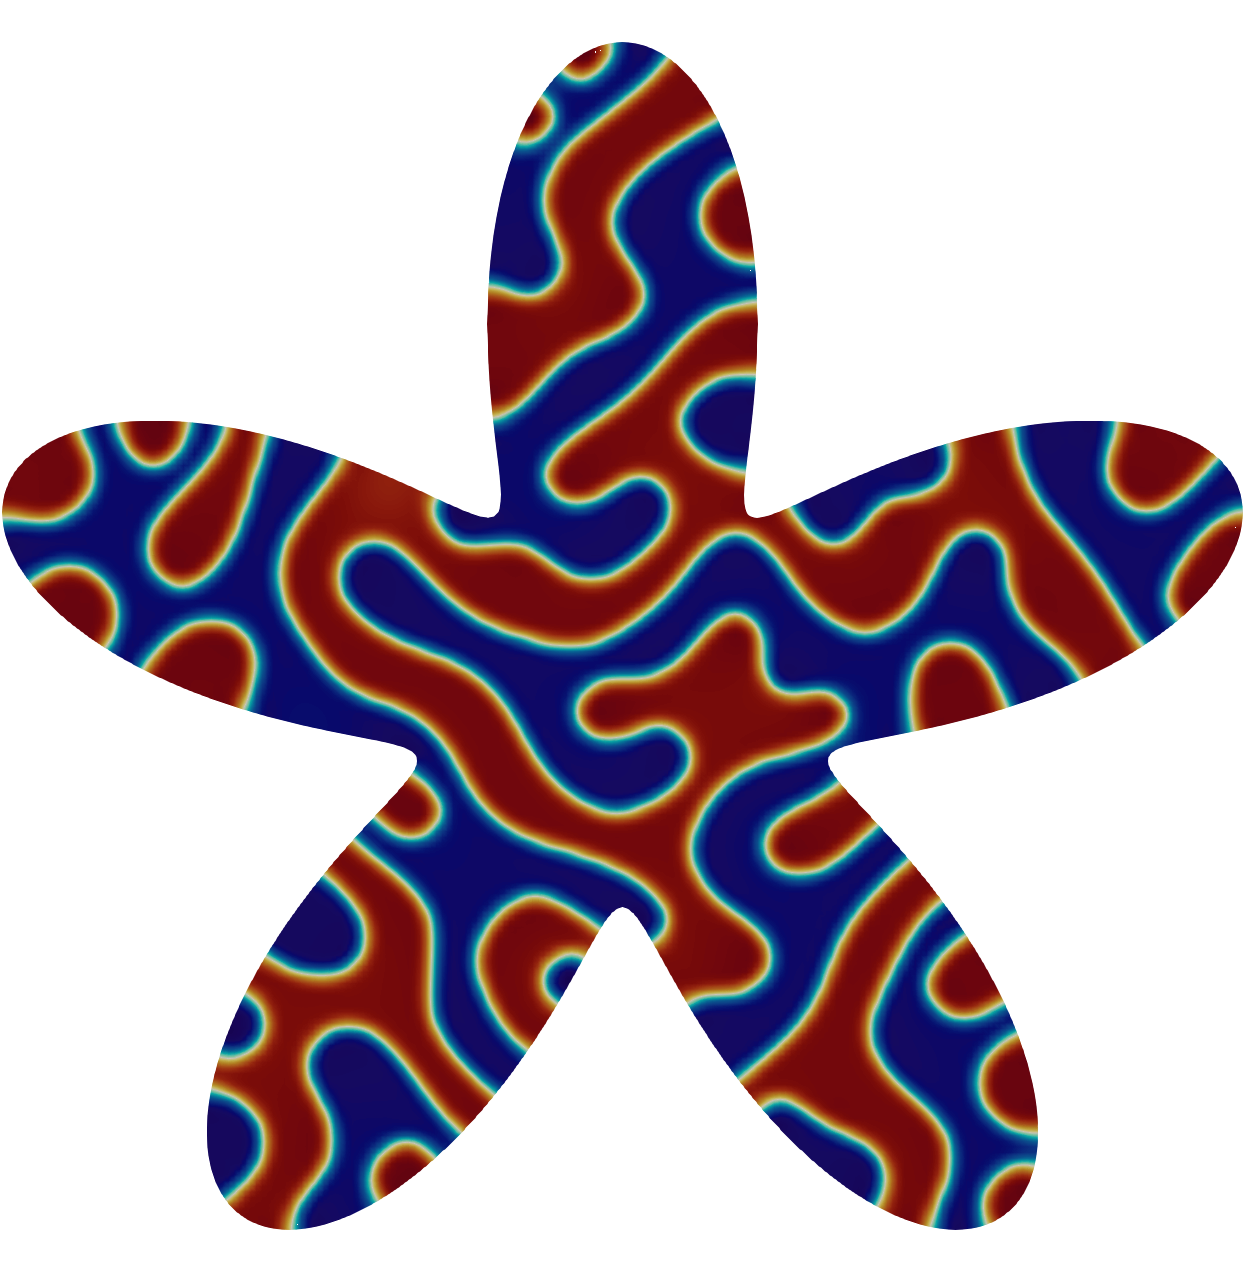
\includegraphics[width=0.5\textwidth]{CH-example/flower_500.png}
    \caption{Iteration 1000}
\end{figure}
\end{frame}

\begin{frame}
\frametitle{The CutCIP Cahn-Hilliard Experiments}
\begin{figure}[h]
    \centering
    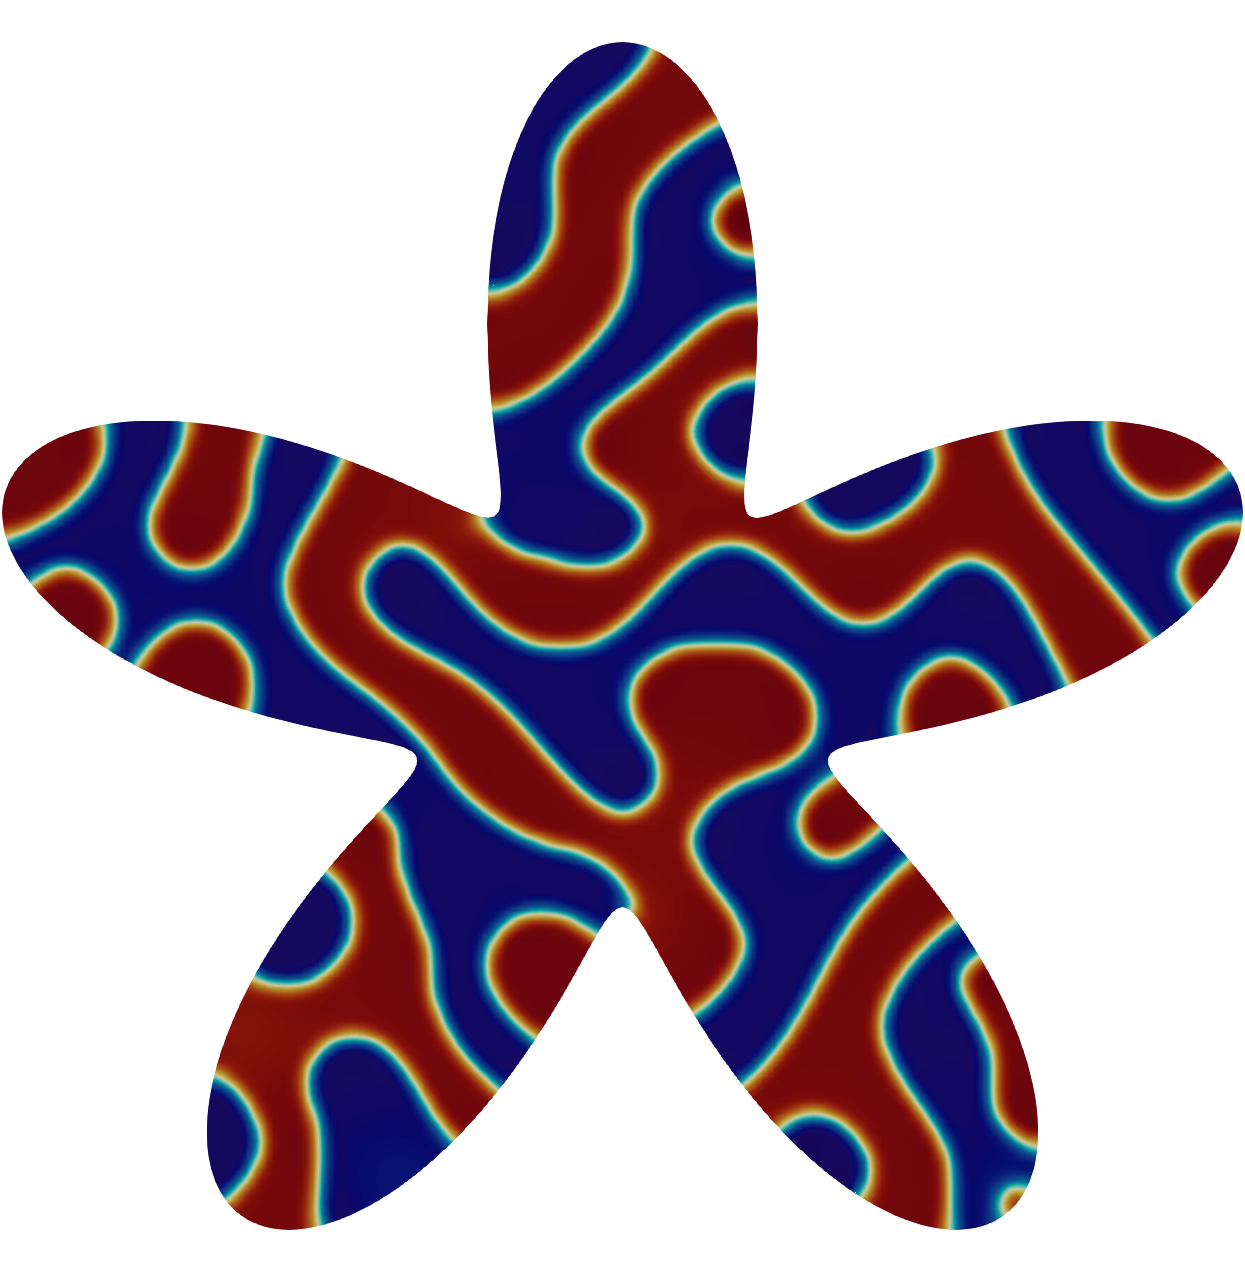
\includegraphics[width=0.5\textwidth]{CH-example/flower_1000.png}
    \caption{Iteration 1000}
\end{figure}
\end{frame}


\begin{frame}
\frametitle{Further work}
\begin{enumerate}
    \item Adaptive time steps.
    \item Further numerical validation.
    \item Extend the method to handle moving domains.

\end{enumerate}
\end{frame}


\begin{frame}
\frametitle{Questions?}
\end{frame}


